\documentclass{standalone}

% For pictures
\usepackage{pgfmath}
\usepackage{tikz}
\usetikzlibrary{shapes, positioning, arrows.meta, patterns, math, decorations.pathreplacing, decorations.pathmorphing}
\definecolor{c3}{RGB}{255, 191, 0} % Amber
\definecolor{c2}{RGB}{86, 193, 255} % Deep Sky Blue
\definecolor{c1}{RGB}{2, 117, 186} % International Klein Blue
\definecolor{c4}{RGB}{130, 233, 70} % Green-Yellow
\definecolor{c5}{RGB}{47, 109, 29} % Army Green


\begin{document}

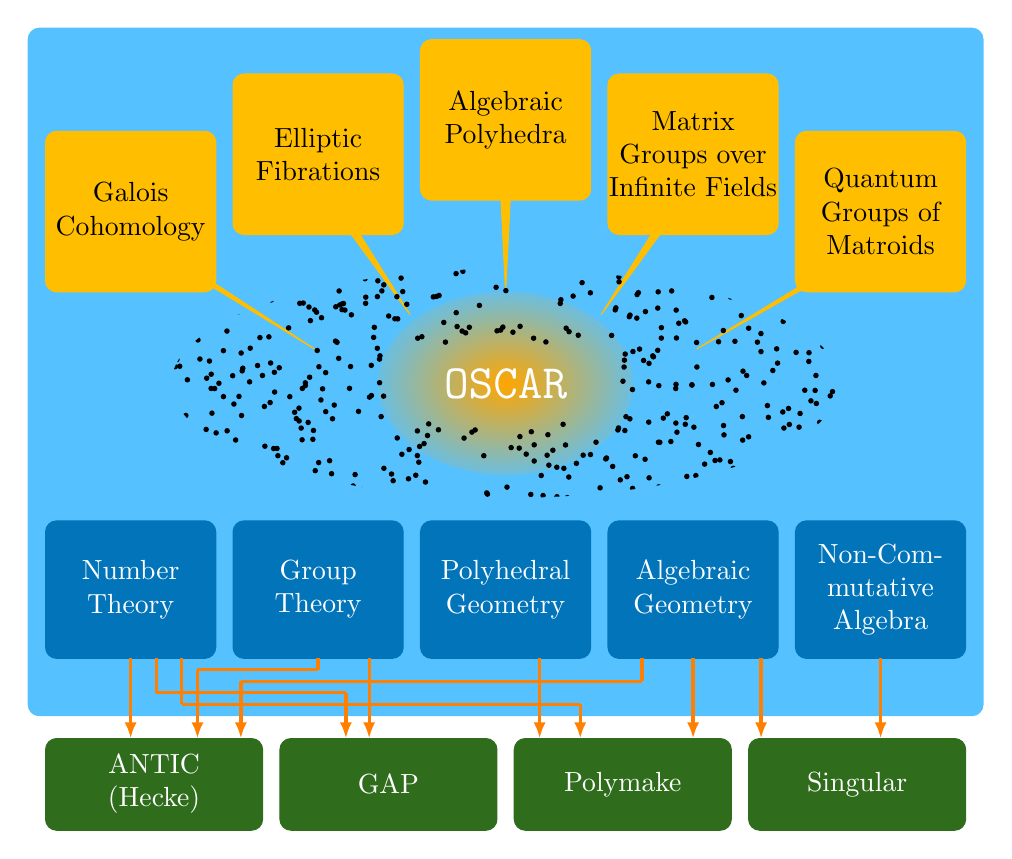
\begin{tikzpicture}

% 1. Define constants
\pgfmathsetlengthmacro{\w}{1.0*\linewidth}
\pgfmathsetlengthmacro{\h}{1.2*\linewidth}
\pgfmathsetlengthmacro{\dd}{\w/55}
\pgfmathsetmacro{\boxwidth}{(\w/5)-(6*\dd/5)}
\pgfmathsetmacro{\secondboxwidth}{(\w/4)-(5*\dd/4)}
\pgfmathsetmacro{\shift}{(-0.02*\h)}

% 2. Draw blue background box
\draw[c2, fill=c2, rounded corners] (0,0.22*\h) rectangle (\w,0.82*\h);

% 3. Zoom out of point cloud to top-layer selling points.
\draw[color = c3, fill = c3] (0.3*\w, 0.54*\h) to (\dd + 0.25*\boxwidth, 0.68*\h+\shift) to (\dd + 0.35*\boxwidth, 0.68*\h+\shift) to (0.3*\w, 0.54*\h);
\draw[color = c3, fill = c3] (0.4*\w, 0.57*\h) to (2*\dd + 1.35*\boxwidth, 0.73*\h+\shift) to (2*\dd + 1.45*\boxwidth, 0.73*\h+\shift) to (0.4*\w, 0.57*\h);
\draw[color = c3, fill = c3] (0.5*\w, 0.59*\h) to (3*\dd + 2.45*\boxwidth, 0.76*\h+\shift) to (3*\dd + 2.55*\boxwidth, 0.76*\h+\shift) to (0.5*\w, 0.59*\h);
\draw[color = c3, fill = c3] (0.6*\w, 0.57*\h) to (4*\dd + 3.55*\boxwidth, 0.73*\h+\shift) to (4*\dd + 3.65*\boxwidth, 0.73*\h+\shift) to (0.6*\w, 0.57*\h);
\draw[color = c3, fill = c3] (0.7*\w, 0.54*\h) to (5*\dd + 4.75*\boxwidth, 0.68*\h+\shift) to (5*\dd + 4.85*\boxwidth, 0.68*\h+\shift) to (0.7*\w, 0.54*\h);

% 4. Draw top-layer selling points of OSCAR
\draw[c3, fill=c3, rounded corners] (\dd + \boxwidth-\boxwidth, 0.75*\h+\shift) rectangle (\dd + \boxwidth, 0.61*\h+\shift);
\draw[c3, fill=c3, rounded corners] (2*\dd + 2*\boxwidth-\boxwidth, 0.80*\h+\shift) rectangle (2*\dd + 2*\boxwidth, 0.66*\h+\shift);
\draw[c3, fill=c3, rounded corners] (3*\dd + 3*\boxwidth-\boxwidth, 0.83*\h+\shift) rectangle (3*\dd + 3*\boxwidth, 0.69*\h+\shift);
\draw[c3, fill=c3, rounded corners] (4*\dd + 4*\boxwidth-\boxwidth, 0.80*\h+\shift) rectangle (4*\dd + 4*\boxwidth, 0.66*\h+\shift);
\draw[c3, fill=c3, rounded corners] (5*\dd + 5*\boxwidth-\boxwidth, 0.75*\h+\shift) rectangle (5*\dd + 5*\boxwidth, 0.61*\h+\shift);
\node[text width=\boxwidth, align=center] at (\dd + 0.5*\boxwidth, 0.68*\h+\shift) {Galois Cohomology};
\node[text width=\boxwidth, align=center] at (2*\dd + 1.5*\boxwidth, 0.73*\h+\shift) {Elliptic Fibrations};
\node[text width=\boxwidth, align=center] at (3*\dd + 2.5*\boxwidth, 0.76*\h+\shift) {Algebraic Polyhedra};
\node[text width=\boxwidth, align=center] at (4*\dd + 3.5*\boxwidth, 0.73*\h+\shift) {Matrix Groups over Infinite Fields};
\node[text width=\boxwidth, align=center] at (5*\dd + 4.5*\boxwidth, 0.68*\h+\shift) {Quantum Groups of Matroids};

% 5. Draw boxes for central topics of OSCAR
\foreach \x in {1,2,3,4,5} {
    \draw[c1, fill=c1, rounded corners] (\x*\dd + \x*\boxwidth-\boxwidth, 0.39*\h) rectangle (\x*\dd + \x*\boxwidth, 0.27*\h);
}
\node[text width=\boxwidth, align=center, color = white] at (\dd + 0.5*\boxwidth, 0.33*\h) {Number Theory};
\node[text width=\boxwidth, align=center, color = white] at (2*\dd + 1.5*\boxwidth, 0.33*\h) {Group Theory};
\node[text width=\boxwidth, align=center, color = white] at (3*\dd + 2.5*\boxwidth, 0.33*\h) {Polyhedral Geometry};
\node[text width=\boxwidth, align=center, color = white] at (4*\dd + 3.5*\boxwidth, 0.33*\h) {Algebraic Geometry};
\node[text width=\boxwidth, align=center, color = white] at (5*\dd + 4.5*\boxwidth, 0.33*\h) {Non-Com-\\mutative Algebra};

% 6. Draw boxes for cornerstones of OSCAR
\foreach \x in {1,2,3,4} {
    \draw[c5, fill=c5, rounded corners] (\x*\dd + \x*\secondboxwidth-\secondboxwidth, 0.20*\h) rectangle (\x*\dd + \x*\secondboxwidth, 0.12*\h);
}
\node[text width=\boxwidth, align=center, color = white] at (\dd + 0.5*\secondboxwidth, 0.16*\h) {ANTIC (Hecke)};
\node[text width=\boxwidth, align=center, color = white] at (2*\dd + 1.5*\secondboxwidth, 0.16*\h) {GAP};
\node[text width=\boxwidth, align=center, color = white] at (3*\dd + 2.5*\secondboxwidth, 0.16*\h) {Polymake};
\node[text width=\boxwidth, align=center, color = white] at (4*\dd + 3.5*\secondboxwidth, 0.16*\h) {Singular};

% % 7. Draw 2nd layer boxes for cornerstones of OSCAR
% \foreach \x in {2,3,4} {
%     \draw[c5, fill=c5, rounded corners] (\x*\dd + \x*\secondboxwidth-\secondboxwidth, 0.08*\h) rectangle (\x*\dd + \x*\secondboxwidth, 0.0*\h);
% }
% \node[text width=\boxwidth, align=center, color = white] at (2*\dd + 1.5*\secondboxwidth, 0.04*\h) {GAP};
% \node[text width=\boxwidth, align=center, color = white] at (3*\dd + 2.5*\secondboxwidth, 0.04*\h) {polymake};
% \node[text width=\boxwidth, align=center, color = white] at (4*\dd + 3.5*\secondboxwidth, 0.04*\h) {Singular};

% 9. Draw flow chart arrows leading off from Number Theory
\draw[very thick, orange, -{Latex[scale=0.7]}] (\dd + 0.5*\boxwidth, 0.27*\h) -- (\dd + 0.5*\boxwidth, 0.2*\h);

\draw[very thick, orange] (1*\dd + 0.5*\boxwidth + 0.15*\boxwidth, 0.27*\h) -- (1*\dd + 0.5*\boxwidth + 0.15*\boxwidth, 0.24*\h);
\draw[very thick, orange] (1*\dd + 0.5*\boxwidth + 0.15*\boxwidth, 0.24*\h) -- (2*\dd + 1.5*\secondboxwidth - 0.25*\boxwidth, 0.24*\h);
\draw[very thick, orange, -{Latex[scale=0.7]}] (2*\dd + 1.5*\secondboxwidth - 0.25*\boxwidth, 0.24*\h) -- (2*\dd + 1.5*\secondboxwidth - 0.25*\boxwidth, 0.2*\h);

\draw[very thick, orange] (1*\dd + 0.5*\boxwidth + 0.3*\boxwidth, 0.27*\h) -- (1*\dd + 0.5*\boxwidth + 0.30*\boxwidth, 0.23*\h);
\draw[very thick, orange] (1*\dd + 0.5*\boxwidth + 0.3*\boxwidth, 0.23*\h) -- (3*\dd + 2.5*\secondboxwidth - 0.25*\boxwidth, 0.23*\h);
\draw[very thick, orange, -{Latex[scale=0.7]}] (3*\dd + 2.5*\secondboxwidth - 0.25*\boxwidth, 0.23*\h) -- (3*\dd + 2.5*\secondboxwidth - 0.25*\boxwidth, 0.2*\h);

% 10. Draw flow chart arrows leading off from Group Theory
\draw[very thick, orange, -{Latex[scale=0.7]}] (2*\dd + 1.8*\boxwidth, 0.27*\h) -- (2*\dd + 1.8*\boxwidth, 0.2*\h);

\draw[very thick, orange] (2*\dd + 1.5*\boxwidth, 0.27*\h) -- (2*\dd + 1.5*\boxwidth, 0.26*\h);
\draw[very thick, orange] (2*\dd + 1.5*\boxwidth, 0.26*\h) -- (\dd + 0.5*\secondboxwidth + 0.2*\secondboxwidth, 0.26*\h);
\draw[very thick, orange, -{Latex[scale=0.7]}] (\dd + 0.5*\secondboxwidth + 0.2*\secondboxwidth, 0.26*\h) -- (\dd + 0.5*\secondboxwidth + 0.2*\secondboxwidth, 0.2*\h);

% 11. Draw flow chart arrows leading off from Tropical Geometry
\draw[very thick, orange, -{Latex[scale=0.7]}] (3*\dd + 2.7*\boxwidth, 0.27*\h) -- (3*\dd + 2.7*\boxwidth, 0.2*\h);

% 12. Draw flow chart arrows leading off from Tropical Geometry
\draw[very thick, orange, -{Latex[scale=0.7]}] (4*\dd + 3.5*\boxwidth, 0.27*\h) -- (4*\dd + 3.5*\boxwidth, 0.2*\h);

\draw[very thick, orange, -{Latex[scale=0.7]}] (4*\dd + 3.9*\boxwidth, 0.27*\h) -- (4*\dd + 3.9*\boxwidth, 0.2*\h);

\draw[very thick, orange] (4*\dd + 3.2*\boxwidth, 0.27*\h) -- (4*\dd + 3.2*\boxwidth, 0.25*\h);
\draw[very thick, orange] (4*\dd + 3.2*\boxwidth, 0.25*\h) -- (\dd + 0.9*\secondboxwidth, 0.25*\h);
\draw[very thick, orange, -{Latex[scale=0.7]}] (\dd + 0.9*\secondboxwidth, 0.25*\h) -- (\dd + 0.9*\secondboxwidth, 0.2*\h);

% 13. Draw flow chart arrows leading off from Non-Commutative Algebra and Free Probability Theory
\draw[very thick, orange, -{Latex[scale=0.7]}] (5*\dd + 4.5*\boxwidth, 0.27*\h) -- (5*\dd + 4.5*\boxwidth, 0.2*\h);

%% 14. Draw flow chart arrows leading off from .jl packages to Cornerstones
%\draw[very thick, orange, -{Latex[scale=2.5]}] (2*\dd + 1.5*\secondboxwidth, 0.12*\h) -- (2*\dd + 1.5*\secondboxwidth, 0.08*\h);
%\draw[very thick, orange, -{Latex[scale=2.5]}] (3*\dd + 2.5*\secondboxwidth, 0.12*\h) -- (3*\dd + 2.5*\secondboxwidth, 0.08*\h);
%\draw[very thick, orange, -{Latex[scale=2.5]}] (4*\dd + 3.5*\secondboxwidth, 0.12*\h) -- (4*\dd + 3.5*\secondboxwidth, 0.08*\h);

% 15. Shade transition in the center
\pgfdeclareradialshading{gradshading}{\pgfpoint{0cm}{0cm}} {rgb(0cm)=(1,0.65,0); rgb(1cm)=(0.34,0.76,1)}
\pgfmathsetmacro{\a}{0.75*\boxwidth}
\pgfmathsetmacro{\b}{0.08*\h}
\shade[shading=gradshading, rounded corners] (0.5*\w, 0.51*\h) ellipse (\a pt and \b pt);

% 16. Draw point cloud to symbolize all other selling points that we cannot talk about.
\pgfmathsetmacro{\cx}{0.5*\dimexpr\w}
\pgfmathsetmacro{\cy}{0.51*\dimexpr\h}
\pgfmathsetmacro{\a}{0.35*\dimexpr\w}
\pgfmathsetmacro{\b}{0.1*\dimexpr\h}
\begin{scope}
\clip (\cx pt,\cy pt) ellipse (\a pt and \b pt);
\foreach \i in {1,...,500}{
    \pgfmathsetmacro{\s}{rand}
    \pgfmathsetmacro{\t}{rand}
    \pgfmathsetmacro{\absS}{abs(\s)}
    \pgfmathsetmacro{\absT}{abs(\t)}
    \pgfmathparse{\absS>0.35 || \absT>0.35}
    \ifnum\pgfmathresult=1
        \fill (\cx pt + \s * \a pt, \cy pt + \t * \b pt) circle (1pt);
    \fi
}
\end{scope}

% 17. Add OSCAR text in the center
\node[align=center, color=white, very thick] at (0.5*\w, 0.51*\h) {\LARGE \texttt{OSCAR}};

\end{tikzpicture}

\end{document}
